\documentclass[tikz, border=5pt]{standalone}

% Semantic GitHub colors for the light theme.
% The Poe task embeds the dark palette from theme-dark.css into each SVG.
\usepackage{tikz}
\usepackage{amsmath, amssymb}
\usetikzlibrary{arrows.meta, calc, positioning, decorations.pathreplacing}

% Text and surfaces.
\definecolor{ghtext}{HTML}{1F2328}
\definecolor{ghmuted}{HTML}{59636E}
\definecolor{ghborder}{HTML}{D1D9E0}
\definecolor{ghpanel}{HTML}{F6F8FA}

% Accent colors and their softer backgrounds.
\definecolor{ghblue}{HTML}{0969DA}
\definecolor{ghbluesoft}{HTML}{DDF4FF}
\definecolor{ghgreen}{HTML}{1A7F37}
\definecolor{ghgreensoft}{HTML}{DAFBE1}
\definecolor{ghpurple}{HTML}{8250DF}
\definecolor{ghpurplesoft}{HTML}{FBEFFF}
\definecolor{ghorange}{HTML}{9A6700}
\definecolor{ghorangesoft}{HTML}{FFF8C5}
\definecolor{ghred}{HTML}{CF222E}
\definecolor{ghredsoft}{HTML}{FFEBE9}

\tikzset{
    >={Stealth[length=2.1mm, width=1.2mm]},
    card/.style={
        fill=ghpanel,
        draw=ghborder,
        rounded corners=2.6mm,
        line width=0.6pt,
    },
    heading/.style={font=\sffamily\small\bfseries, text=ghtext},
    regular/.style={font=\sffamily\small, text=ghtext},
    note/.style={font=\sffamily\footnotesize, text=ghmuted},
    tinylabel/.style={font=\sffamily\scriptsize, text=ghmuted},
    mathlabel/.style={font=\sffamily\small, text=ghtext},
    bluearrow/.style={-Stealth, draw=ghblue, line width=1.5pt},
    purplearrow/.style={-Stealth, draw=ghpurple, line width=1.4pt},
    thin/.style={draw=ghborder, line width=0.7pt},
}


\begin{document}
    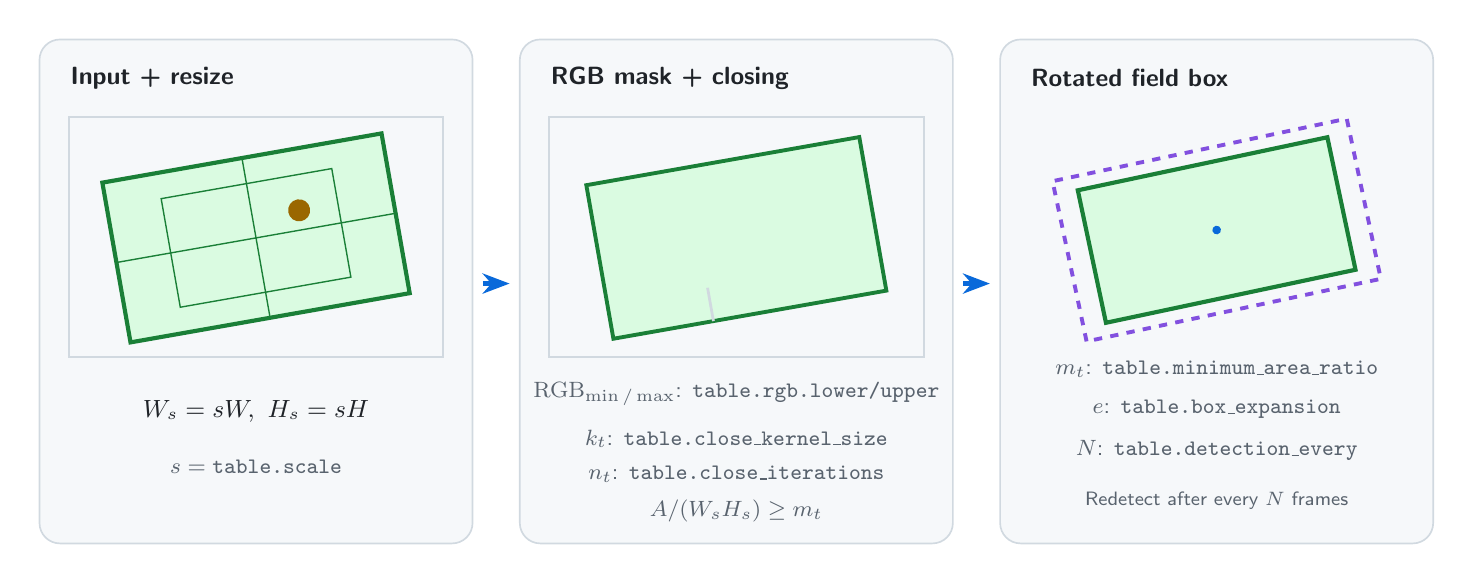
\begin{tikzpicture}[x=1cm, y=1cm]
        \path[use as bounding box] (0, 0) rectangle (18, 6.7);

        % Three processing stages.
        \draw[card] (0.15, 0.15) rectangle (5.65, 6.55);
        \draw[card] (6.25, 0.15) rectangle (11.75, 6.55);
        \draw[card] (12.35, 0.15) rectangle (17.85, 6.55);

        \node[heading, anchor=west] at (0.42, 6.06) {Input + resize};
        \node[heading, anchor=west] at (6.52, 6.06) {RGB mask + closing};
        \node[heading, anchor=west] at (12.62, 6.06) {Rotated field box};

        % Frame dimensions and resized coordinates.
        \draw[thin] (0.52, 2.52) rectangle (5.28, 5.56);
        \begin{scope}[shift={(2.9, 4.03)}, rotate=10]
            \fill[ghgreensoft] (-1.8, -1.03) rectangle (1.8, 1.03);
            \draw[ghgreen, line width=1.5pt]
                (-1.8, -1.03) rectangle (1.8, 1.03);
            \draw[ghgreen, line width=0.5pt]
                (0, -1.03) -- (0, 1.03)
                (-1.8, 0) -- (1.8, 0);
            \draw[ghgreen, line width=0.5pt]
                (-1.1, -0.7) rectangle (1.1, 0.7);
            \fill[ghorange] (0.6, 0.25) circle (0.14);
        \end{scope}

        \node[mathlabel] at (2.9, 1.83) {$W_s=sW,\ H_s=sH$};
        \node[note] at (2.9, 1.13) {$s=\texttt{table.scale}$};

        % Color mask and morphological closing.
        \draw[thin] (6.62, 2.52) rectangle (11.38, 5.56);
        \begin{scope}[shift={(9, 4.03)}, rotate=10]
            \fill[ghgreensoft] (-1.76, -0.99) rectangle (1.76, 0.99);
            \draw[ghgreen, line width=1.4pt]
                (-1.76, -0.99) rectangle (1.76, 0.99);
            \draw[ghborder, line width=1pt]
                (-0.47, -0.99) -- (-0.47, -0.56);
        \end{scope}

        \node[note] at (9, 2.05)
            {$\mathrm{RGB}_{\min/\max}$: \texttt{table.rgb.lower/upper}};
        \node[note] at (9, 1.48)
            {$k_t$: \texttt{table.close\_kernel\_size}};
        \node[note] at (9, 1.03)
            {$n_t$: \texttt{table.close\_iterations}};
        \node[note] at (9, 0.56)
            {$A/(W_sH_s)\geq m_t$};

        % Minimum-area rectangle, expansion, and refresh period.
        \begin{scope}[shift={(15.1, 4.13)}, rotate=12]
            \fill[ghgreensoft] (-1.62, -0.86) rectangle (1.62, 0.86);
            \draw[ghgreen, line width=1.5pt]
                (-1.62, -0.86) rectangle (1.62, 0.86);
            \draw[ghpurple, dashed, line width=1.4pt]
                (-1.91, -1.04) rectangle (1.91, 1.04);
            \fill[ghblue] (0, 0) circle (0.055);
        \end{scope}

        \node[note] at (15.1, 2.36)
            {$m_t$: \texttt{table.minimum\_area\_ratio}};
        \node[note] at (15.1, 1.85)
            {$e$: \texttt{table.box\_expansion}};
        \node[note] at (15.1, 1.33)
            {$N$: \texttt{table.detection\_every}};
        \node[tinylabel] at (15.1, 0.69)
            {Redetect after every $N$ frames};

        % Processing flow.
        \draw[bluearrow] (5.78, 3.45) -- (6.12, 3.45);
        \draw[bluearrow] (11.88, 3.45) -- (12.22, 3.45);
    \end{tikzpicture}
\end{document}
